\documentclass[11pt]{article}
\usepackage[final]{acl}
\usepackage{times,latexsym}
\usepackage[T1]{fontenc}
\usepackage[utf8]{inputenc}
\usepackage{microtype,amsmath,amssymb,booktabs,graphicx,array,multirow}
\usepackage{xurl}
\graphicspath{{../figures/}}
\renewcommand{\dbltopfraction}{0.82}
\setcounter{dbltopnumber}{3}
\newcommand{\G}{\mathsf{G}}
\newcommand{\W}{\mathbf{W}}
\title{WELD: How Well Do Language Models\\Build and Adapt Dynamic Workflows?}
\author{Zhixuan Liu \\ Northeastern University
\And Qi Yan\thanks{Corresponding author.} \\ Northeastern University}
\begin{document}
\maketitle
\begin{abstract}
Language models increasingly decide what work an agent system performs, how results are combined, and what must change when requirements evolve. Evaluating the final answer alone leaves these decisions largely unmeasured. We introduce WELD, an executable benchmark of workflow effectiveness that connects task validity, domain-native work, realized time savings, and selective adaptation. Its 100 parent tasks span five scenarios and 20 source clusters, with initial, relevant-change, and irrelevant-change conditions. Ten API-served models produce 6,000 evaluated stages; fixed-response replay adds 8,874 native executions. Among 5,006 pairs of valid initial solutions, 2,241 exhibit work dominance and 372 exhibit resource trade-offs. Equal tool-call counts conceal unequal primary work in 187 pairs. For medium tasks, online time savings fall below work savings by an equal-parent mean of 31.6 percentage points, falling to 14.5 after removing local admission waits. Native replay often realizes the savings. Following valid initial results, models preserve validity in 99.3\% of irrelevant changes but only 54.6\% of relevant changes. WELD makes workflow effectiveness measurable as a profile of successful work, realized benefit, and maintenance behavior.
\end{abstract}

\section{Introduction}
An agent's workflow determines what it reads, which tests it runs, what it shares, and what it repeats. Two models can return the same correct answer while making very different choices along the way. One query can scan a small requested population or aggregate an entire database. A reused observation can save a tool call or silently preserve a result from the wrong version. The final answer tells us whether the task was solved. It does not tell us how effectively the work was organized.

Recent benchmarks have made workflow execution a concrete object of evaluation. In particular, ClawArena-Team fixes the worker pool and evaluates the model acting as manager through execution-based task, permission, and modality-routing scores \citep{xiong2026clawarenateam}. This is an important step: the model's decisions can be studied while the workers remain controlled. The next measurement problem lies inside the resulting execution. A successful workflow can still request excessive work, fail to turn local savings into faster completion, or lose validity when only part of the task changes. A manager-level score does not resolve these three questions.

We study \emph{workflow effectiveness}: the relationship between runtime decisions, induced work, and maintained results. Work retains its domain meaning; time separates native execution from interaction and waiting; adaptation starts from the model's own completed state. These linked observations make reuse, repair, and realized benefit directly comparable.

We introduce \textbf{WELD}, \emph{Work, Execution, and Lifecycle Diagnostics}. Models iteratively create dataflows; fixed native workers execute batches and return observations. Executable contracts check results and supporting evidence or state. Versioned artifacts, revisions, and execution events connect intention to behavior, supporting three comparisons: work among valid solutions, work savings versus time savings, and relevant versus irrelevant changes.

The benchmark contains 100 parents from 20 source clusters across five scenarios. Easy and medium tasks preserve choices about batching, scope, reuse, and integration while providing a substantial valid comparison pool. The study covers ten models, 6,000 stages, and 8,874 faithful native replays.

Successful workflows differ in native work even at equal call counts. Native savings can be attenuated online. Preserving a result under an irrelevant notice is easier than repairing it after a relevant change. WELD provides executable tasks, measurement rules, and trace-level evidence to study these gaps together.

\section{Related Work}
\paragraph{Workflow evaluation.}
WorFBench introduces diverse workflow-generation tasks and subsequence/subgraph matching, with downstream performance and timing experiments \citep{qiao2025worfbench}. Structural agreement does not specify how much native work a valid alternative performs. FlowMind separates task execution from workflow reconstruction and introduces FlowBench \citep{liu2026flowmind}. It establishes an execution-grounded route to structured workflows; our comparison starts with the executed alternatives and follows their resource use and later revisions. OrchBench evaluates assignments and information transfer over given DAGs with a deterministic quality, makespan, and token simulator \citep{ren2026orchbench}. WELD lets models discover executable investigations and measures their native operations and observed time.

\paragraph{Agent evaluation.}
AgentBoard provides progress-rate measurement and analytical tools for multi-turn agents \citep{agentboard}. Progress toward subgoals is complementary to the amount of work needed to reach them. AppWorld supplies executable applications and state-based tests that admit multiple solutions \citep{trivedi2024appworld}. WELD adopts outcome-based validation and adds paired workload measurement and completed-state changes across five domains. ClawArena-Team isolates management with controlled workers and measures permissions, modality routing, and task success \citep{xiong2026clawarenateam}. Its API cost analysis demonstrates that expense and quality can diverge. We examine a different link: whether measured native savings are realized online, and how much valid state survives a change.

\paragraph{Efficiency and evaluation units.}
\citet{agentsmatter} argue for joint accuracy--cost evaluation, reproducibility, and better holdout design. BIRD measures SQL execution quality and efficiency on realistic databases \citep{bird}. These establish efficiency as a necessary evaluation axis. WELD connects a vector of observed work to time and update behavior within the same execution record. Table~\ref{tab:coverage} summarizes the specific protocols compared here.


\section{WELD: Executable Measurement}
\subsection{A model-created, evolving dataflow}
A task is $(x,c,\mathcal{O},V)$: a frozen source world $x$, a public contract $c$, permitted operators $\mathcal{O}$, and an executable validator $V$. At round $t$, the model sees the task, current nodes, versioned observations, and execution feedback. It proposes nodes containing an operator, arguments, and dependencies. Arguments may reference prior outputs. The runtime executes a selected batch and returns its observations before the next decision. The model can then create investigations, revise pending scopes, add dependencies, or submit a result. The workflow is constructed through these decisions rather than supplied as a fixed DAG.

Four deterministic worker slots execute native operators. Domain adapters expose graph traversal, source reads and regression probes, read-only SQL, telemetry queries, and local application-state transitions. Shared transformations implement filtering, grouping, projection, sorting, and aggregation. Models can use native aggregate operators or compose lower-level operations. Long outputs remain available through references even when their displayed preview is truncated.

The runtime stores three separate records: the initial graph, subsequent revisions, and actual execution events. Each artifact records its producer, input artifacts, source version, and content hash. Update stages inherit the completed checkpoint; inherited work retains its identity and is excluded from incremental resource totals. Figure~\ref{fig:design} connects these records to the three evaluation questions.

\begin{figure*}[t]
\centering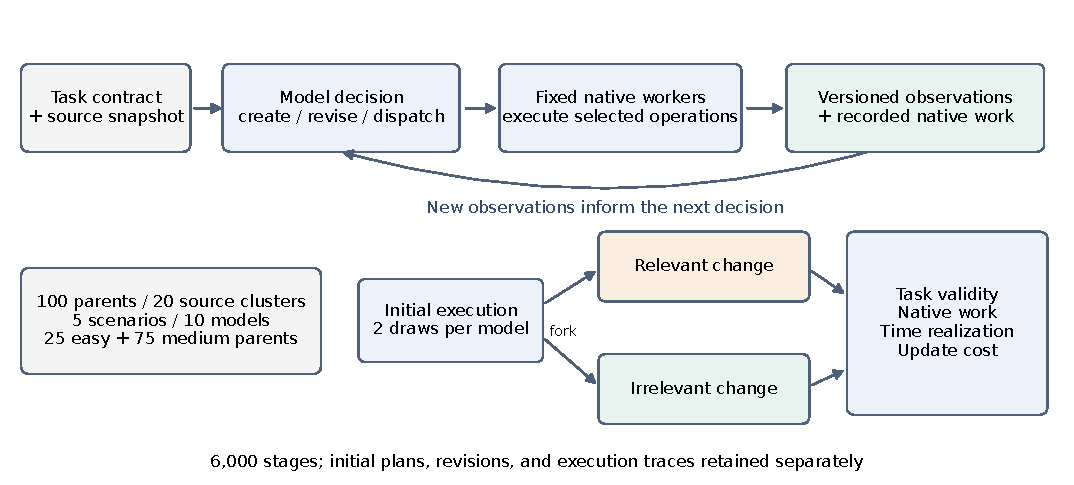
\includegraphics[width=.95\textwidth]{figure_0_experiment_design.pdf}
\caption{WELD's execution and measurement protocol. The model receives observations between dispatch batches and determines subsequent work. Relevant and irrelevant conditions branch from the same initial checkpoint. Native replay fixes model responses and varies worker capacity.}
\label{fig:design}
\end{figure*}

\subsection{Validity and the comparison population}
For a submitted result $y$, observations $E$, and final state $s$, define
\begin{align}
Q_1&=\mathbb{1}[y,s\text{ satisfy the output contract}],\\
Q_2&=\mathbb{1}[E,s\text{ satisfy support requirements}],\\
\G&=Q_1Q_2.\label{eq:gate}
\end{align}
Read-only tasks check required values, entity or test identities, and applicable observations. Business tasks check the resulting state and required preservation. Alternative decompositions can pass the same contract. A frozen equivalence audit admits equivalent SQL and graph access paths. Supporting artifacts are attached automatically, so evidence validity evaluates executed support rather than citation formatting.

Every planned stage contributes to unconditional validity. A missing submission contributes zero. Work--time comparisons additionally require both executions to pass $\G$ on the same parent, initial condition, and generation index. We report this comparison pool alongside success rates. Thus a model that rarely succeeds receives a low unconditional score and supplies fewer eligible comparisons.

\subsection{Work and time accounting}
Let $\mathcal{E}_\tau$ contain the uniquely identified executed events of workflow $\tau$. Its work vector is
\begin{equation}
\W(\tau)=\sum_{e\in\mathcal{E}_\tau}\mathbf{w}(e).
\label{eq:work}
\end{equation}
Coordinates retain native units: examined graph records, executed regression cases, database progress callbacks, metric values, scanned log and trace rows, application records and writes, and transformations. Tool and worker attempts, including failures, are also recorded. Model requests have a separate ledger containing input/output usage, charge receipts, unknown charges, and retries.

For workflow $a$ to dominate $b$ in recorded native work,
\begin{equation}
\begin{aligned}
&\forall j\in J:W_j(a)\le W_j(b),\\
&\exists j\in J:W_j(a)<W_j(b).
\end{aligned}
\label{eq:dominance}
\end{equation}
$J$ includes every active native-work coordinate in that scenario and excludes model requests. Equal vectors and trade-offs are retained separately. No conversion between cases, records, and writes is needed.

Online elapsed time $T$ covers runtime start through completion, including model requests and local admission waits. Validation runs afterward. If $U_M$ and $U_W$ are unions of model-request and worker intervals, with overlap $O$, then
\begin{equation}
T=U_M+U_W-O+T_{\mathrm{other}}.
\end{equation}
We also report online time minus measured local admission waits. Provider waiting remains in this quantity. Native replay feeds back the saved model responses without API calls and repeats native execution with one and four worker slots. Its timing statistic is the union of worker-active intervals, summarized by the median of three replays. This measures the native execution layer; online time measures completion of the interactive workflow.

For a dominating low-work execution $\ell$ and its higher-work counterpart $h$, we use a declared primary coordinate $j_s$ for scenario $s$:
\begin{equation}
S_W=1-\frac{W_{j_s}(\ell)}{W_{j_s}(h)},\qquad
S_T=1-\frac{T(\ell)}{T(h)}.
\label{eq:savings}
\end{equation}
Eligible pairs have unequal primary work, positive denominators, and one physical attempt per stage. The work--time gap $D=S_W-S_T$ is positive when savings are attenuated. In particular, $0<S_T<S_W$ captures useful but subproportional time savings. Online comparisons additionally match acquisition campaign and admission segment.

\subsection{Selective adaptation and incremental cost}
For update type $u\in\{\mathrm{rel},\mathrm{irr}\}$ and valid initial runs, we measure
\begin{equation}
A_u=\frac{\sum_{p,r}\G_{p,r,0}\G_{p,r,u}}
{\sum_{p,r}\G_{p,r,0}}.
\label{eq:adapt}
\end{equation}
Relevant updates alter requirements, source versions, or source state. Irrelevant updates preserve the requested result. Both branches receive the same initial checkpoint. New events determine $\Delta\W$, $\Delta C$, and $\Delta T$; a complete lifecycle counts the prefix once.

A separate prefix audit evaluates the old answer and old evidence under the new condition. This distinguishes changes requiring a new answer, a new observation, both, or neither. For version-changed read-only sources, the validator can re-execute an inherited observation to test whether its value remains applicable. Such verification work is logged separately and never presented as model work.

\subsection{Aggregation and instrument checks}
The quality table reports $\G$ for each scenario and the equal-scenario mean. Each scenario contributes 20 parents, three conditions, and two repeats. Hence the all-stage macro rate equals the valid count divided by 600 for each model. Initial validity and conditional adaptation are shown separately. Work, time, and adaptation retain their own units and denominators.

Paired observations share parents and model outputs. We first average the work--time gap within each parent and bootstrap parents 4,000 times for a 95\% percentile interval. Adaptation sensitivity additionally resamples source clusters within scenarios and parents within clusters. Pairwise common-support and leave-one-source-out tables accompany the main results.

Acceptance checks exercise positive witnesses, wrong identities, stale versions, alternative representations, and failed execution. Final audits reconcile all logical stages with physical attempts and artifact references. All 8,874 selected native replays reproduce valid outcomes, identical native observations, and identical work vectors. Appendix~\ref{app:properties} states the accounting invariants and their mathematical consequences.

\section{Task Construction}
\label{sec:data}
WELD has five scenarios, each with 20 parent tasks, five easy and fifteen medium. Every parent produces base, relevant-change, and irrelevant-change cards. The resulting 300 cards are evaluated twice per model. Figure~\ref{fig:data} shows the construction and source allocation.

\begin{figure*}[t]
\centering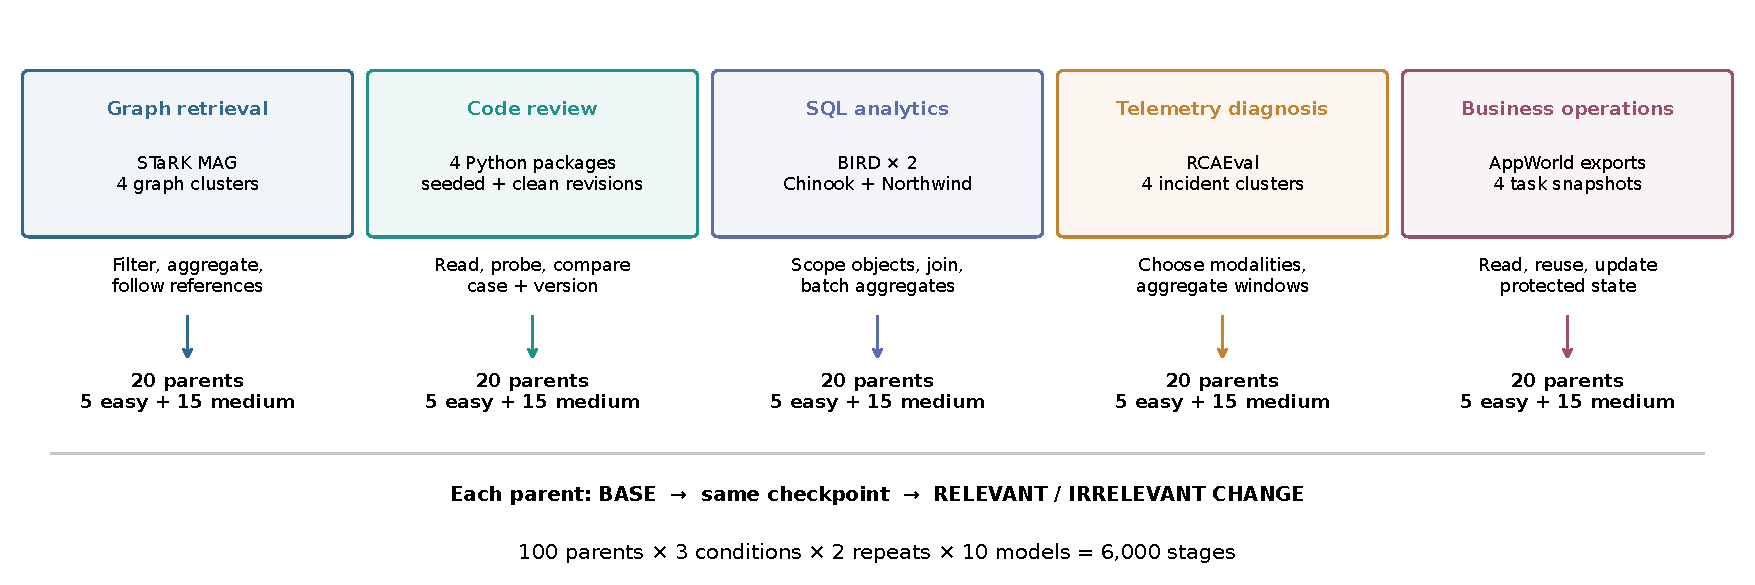
\includegraphics[width=\textwidth]{figure_4_dataset.pdf}
\caption{From frozen sources to paired task conditions. Four source clusters per scenario produce 20 parents. Each parent has one base and two checkpoint-conditioned continuations. Easy and medium tasks vary answer burden while retaining decisions about scope, batching, reuse, and updates.}
\label{fig:data}
\end{figure*}

\paragraph{Graph retrieval.}
We derive compositional queries from STaRK's MAG graph \citep{stark}. The sources comprise an existing shared slice and institution-centered neighborhoods for Stanford, MIT, and the University of Tokyo. Author publication closures and outgoing references are retained. Easy tasks summarize one author's publication count, citations, and top paper. Medium tasks combine authors and retrieve references of a selected top paper. Relevant updates expand the requested year interval from 2010--2014 to 2000--2024. Filtering before aggregation, broad retrieval, and reuse of previously read records lead to different work profiles.

\paragraph{Code review.}
Four pinned Python packages provide executable behavior: Requests 2.32.5, ItsDangerous 2.2.0, packaging 25.0, and python-dotenv 1.1.1 \citep{requests,itsdangerous,packaging,dotenv}. We construct clean and seeded snapshots around redirect or copy behavior, timestamp boundaries, version constraints, and parser behavior. Public registered cases state expected behavior; native probes observe the current snapshot. Models return a verdict and the exact failing case identities. Medium tasks increase scoped cases and cross-module requirements. A related update changes the implementation revision. These are authored regression-review tasks over upstream code, with seed provenance preserved.

\paragraph{Database analytics.}
BIRD debit and financial databases, Chinook, and Northwind supply four clusters \citep{bird,birdminidev,chinook,northwind}. Tasks request entity-bound aggregates: consumption, regional loan summaries, or customer purchases. Medium cards request more objects and fields. Relevant updates replace a requested object or change a value. Models may use scoped aggregate operators or read-only SQL, allowing batching, broad aggregation, and repeated queries to be compared. Evidence must bind results to the requested entities.

\paragraph{Telemetry diagnosis.}
RCAEval supplies metrics, logs, and traces from Online Boutique and Train Ticket \citep{rcaeval}. We group the original checkout incidents and three additional service incidents into four clusters. Tasks identify the metric with the largest post/pre mean ratio at a public split. Medium cards add trace-duration ratios and log-match counts. Related changes shift the split timestamp while preserving the raw telemetry. These tasks use diagnostic quantities derived from source telemetry, with explicit numerical ground truth.

\paragraph{Business operations.}
Four AppWorld task snapshots provide playlist, user, and payment records \citep{trivedi2024appworld}. We export those records into a local deterministic state adapter and author playlist playback, offline download, and payment reconciliation tasks. Updates change a duration, add a playlist, or apply a partial payment. Multiple playlists can satisfy a duration requirement; prior downloads can be reused; payment writes replace a member's requested total. State tests check requested effects and protected state. The reported scores concern these adapted tasks.

\paragraph{Construction controls.}
Frozen source records generate public task cards and private expected results separately. Requirements specify identities, numeric tolerances, state obligations, and permitted operations. Reference executions check satisfiability and controlled mutations test rejection. Sources, adaptations, hashes, and task memberships are included in the release. The 20 clusters preserve shared-corpus relationships: MAG neighborhoods can share references, and AppWorld snapshots share generated base data. Earlier complex stress tasks remain a separate study.

\section{Experimental Setup}
We evaluate ten API-served models using the same task interface and fixed native workers (Table~\ref{tab:quality}). Every model completes 600 logical stages. Two provider-default generations are collected per card, with 12 decision rounds for initial stages, eight for updates, four worker slots, and at most 8,192 output tokens per decision. Endpoint-compatible reasoning settings are frozen in development and listed in Appendix~\ref{app:models}. The interface uses JSON objects with nodes and a final answer. Format failures, tool failures, and unsubmitted stages remain in the quality denominator.

Collection proceeds across recorded campaigns. Historical results and the final five-model extension share the task contracts and final evidence-equivalence rules. Confirmed transport interruptions can be replaced under the recorded policy; unsuccessful model answers are retained. Work includes physical attempts. Timing pairs use clean stages and matching acquisition conditions. Native replay places all ten models in a common offline campaign with three repeats per worker configuration. Replays from an earlier interrupted disk volume are excluded in full. This yields 6,000 main stages and 8,874 final replay executions.

\section{Results}
\begin{figure*}[t]
\centering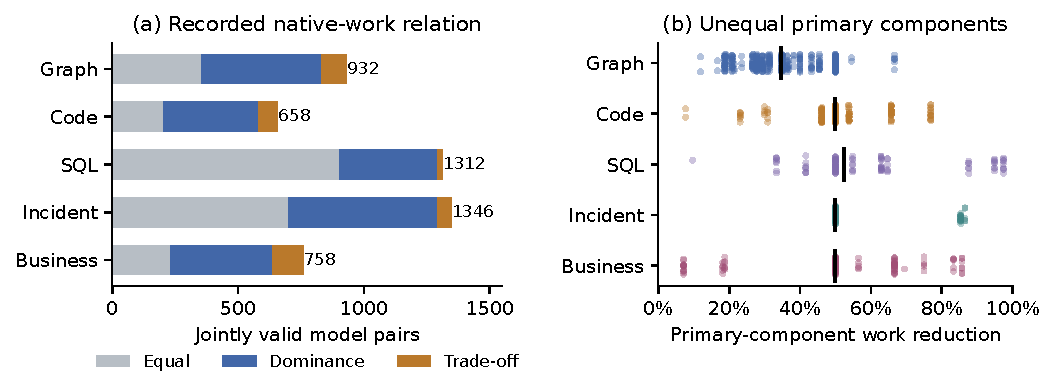
\includegraphics[width=\textwidth]{figure_1_correct_work_differences.pdf}
\caption{Native work among 5,006 paired valid initial executions. Left: equality, dominance, and trade-offs across the complete recorded work vector. Right: differences in each scenario's primary work coordinate. Coordinate-level savings must be read together with the full-vector relation.}
\label{fig:work}
\end{figure*}
\begin{figure*}[t]
\centering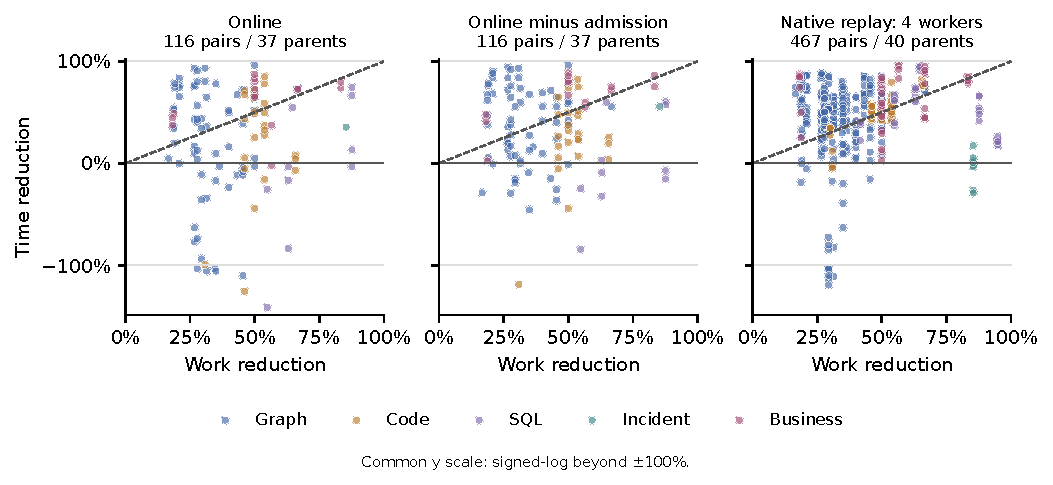
\includegraphics[width=\textwidth]{figure_2_work_to_time.pdf}
\caption{Work savings versus time savings on medium tasks. Online panels contain 116 matched acquisition pairs over 37 parents. Four-worker native replay contains 467 pairs over 40 parents. The diagonal represents proportional realization; positive points below it are useful but attenuated savings. Native timing is worker-active union time.}
\label{fig:time}
\end{figure*}
\begin{figure*}[t]
\centering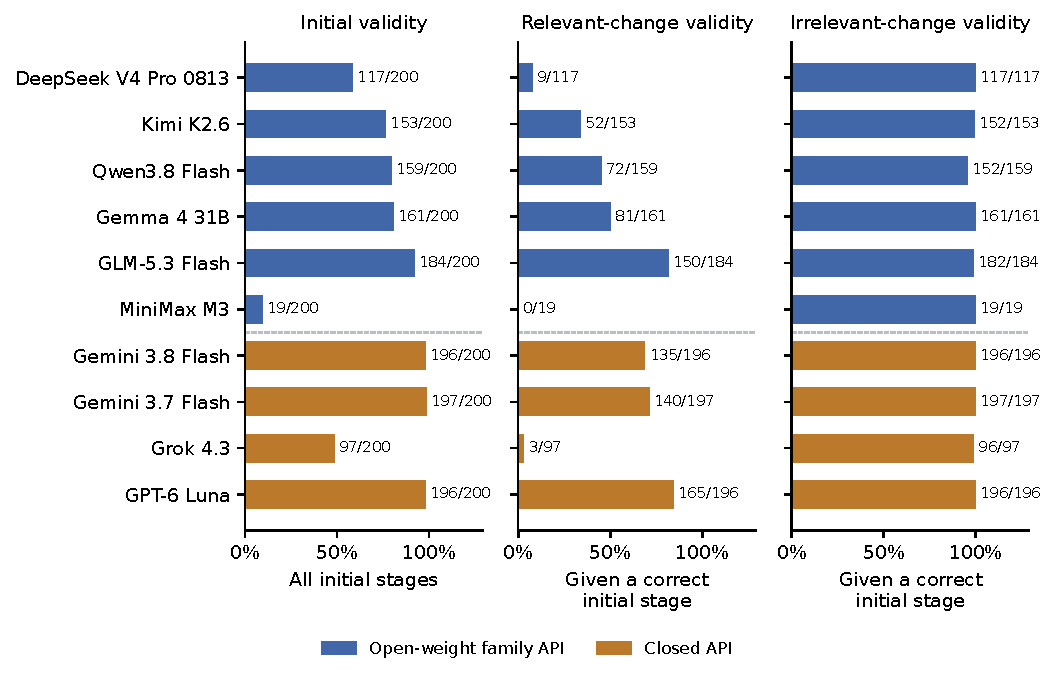
\includegraphics[width=\textwidth]{figure_3_selective_adaptation.pdf}
\caption{Initial validity and adaptation from valid initial states. Related and unrelated bars use the valid-initial denominator printed for each model. The two endpoint-family groups are shown separately; all models are API-served. Conditional bars describe each model's own valid pool. Pairwise common-support comparisons are supplied separately.}
\label{fig:adapt}
\end{figure*}
\subsection{Validity opens a substantial comparison pool}
\begin{table*}[t]
\centering\small\setlength{\tabcolsep}{5pt}
\begin{tabular}{lrrrrrrr}
\toprule
Model & Graph & Code & SQL & Telemetry & Business & All stages & Initial \\
\midrule
\multicolumn{8}{l}{\emph{Open-weight model families, served through APIs}}\\
DeepSeek V4 Pro 0813 & 29.2 & 34.2 & 70.0 & 61.7 & 29.2 & 44.8 & 58.5 \\
Kimi K2.6 & 52.5 & 48.3 & 78.3 & 67.5 & 65.0 & 62.3 & 76.5 \\
Qwen3.8 Flash & 84.2 & 40.0 & 88.3 & 65.8 & 56.7 & 67.0 & 79.5 \\
Gemma 4 31B & 86.7 & 23.3 & 98.3 & 66.7 & 63.3 & 67.7 & 80.5 \\
GLM-5.3 Flash & 97.5 & 63.3 & 92.5 & 86.7 & 98.3 & 87.7 & 92.0 \\
MiniMax M3 & 0.0 & 10.0 & 5.8 & 20.8 & 6.7 & 8.7 & 9.5 \\
\midrule
\multicolumn{8}{l}{\emph{Closed-model APIs}}\\
Gemini 3.8 Flash & 100.0 & 71.7 & 99.2 & 70.8 & 100.0 & 88.3 & 98.0 \\
Gemini 3.7 Flash & 100.0 & 68.3 & 100.0 & 76.7 & 100.0 & 89.0 & \textbf{98.5} \\
Grok 4.3 & 41.7 & 18.3 & 57.5 & 49.2 & 17.5 & 36.8 & 48.5 \\
GPT-6 Luna & 98.3 & 72.5 & 100.0 & 98.3 & 96.7 & \textbf{93.2} & 98.0 \\
\bottomrule
\end{tabular}
\caption{Joint-valid rates (\%). Each scenario column includes 120 stages per model; all stages includes 600, and initial includes 200. The balanced design makes the all-stage rate equal to the equal-scenario macro mean. Bold marks the best all-stage and initial rates. Endpoint-family grouping is descriptive: the Qwen production API is not identified with a specific released checkpoint.}
\label{tab:quality}
\end{table*}
Across all conditions, 3,873 of 6,000 stages pass $\G$. Initial validity is 1,479/2,000 (74.0\%), providing eligible initial comparisons in all 100 parents. The scenario totals are 291/400 for graph retrieval, 235/400 for code review, 343/400 for analytics, 347/400 for telemetry, and 263/400 for business operations. This preserves meaningful difficulty while supporting direct comparisons of valid executions.

Initial validity and lifecycle validity distinguish different strengths. Gemini 3.7 Flash has the highest initial count, 197/200. GPT-6 Luna has the highest all-stage count, 559/600, and the highest observed relevant-update rate, 165/196. GLM-5.3 Flash achieves 150/184 relevant recoveries with a lower initial count. MiniMax M3 yields 19 valid initial stages despite producing submissions for all 600 stages. Submission is therefore a transport/interface outcome, not evidence that the task was solved.

\subsection{Finding 1: equal outcomes conceal different work}

The 1,479 valid initial executions form 5,006 cross-model pairs on matched parent--repeat cells. Of these, 2,393 have equal work vectors, 2,241 exhibit dominance, and 372 exhibit trade-offs (Figure~\ref{fig:work}). Correctness therefore identifies a population within which work remains meaningfully different.

Tool-call count removes part of this variation from view. Among 3,619 pairs with equal call counts, 187 have unequal primary native work, spanning 29 parents. In customer-audit task A14, a Qwen3.8 Flash solution and several valid alternatives each use one native tool call, yet register 39 versus two SQLite progress callbacks. The ratio is 19.5 for this measured proxy. Calling both solutions ``one-query workflows'' hides the difference in database work.

Trade-offs are equally informative. A workflow can reduce one kind of work while increasing another; the 372 incomparable pairs keep these decisions visible. WELD therefore reports the work vector and its relation before calculating a primary-coordinate saving. This gives a concrete answer to which valid workflow is better under a stated resource preference.

\subsection{Finding 2: native savings and online benefit separate}

For medium tasks, 116 dominant-work pairs satisfy the online acquisition controls. Twenty-nine realize positive but attenuated time savings, 33 realize zero or negative savings, and 54 realize at least proportional savings. Averaging the gap $D$ within parents yields 31.6 percentage points (95\% interval: 13.7--52.4). Removing local admission waits reduces this gap to 14.5 points (3.7--26.3). Admission matters, and a positive gap remains after it is removed.

The native layer behaves differently. Among 467 four-worker pairs, 108 show positive attenuation, 27 show nonpositive savings, and 332 realize at least proportional savings. Their equal-parent mean gap is $-6.0$ points, with an interval of $[-13.7,2.9]$. The broader native pool therefore does not show a positive average attenuation gap.

Comparing the same 116 pairs across timing domains resolves the pool difference. Native time savings exceed admission-adjusted online savings by an equal-parent mean of 24.2 points (13.9--34.5). The measurement locates a gap between local execution and interactive completion. Model requests, provider waiting, and runtime coordination can absorb native gains. These observations motivate evaluating batching and interaction frequency alongside the amount of work requested.

\subsection{Finding 3: preservation is easier than repair}

From the 1,479 valid initial states, irrelevant changes preserve validity in 1,468 cases (99.3\%). Relevant changes yield only 807 valid continuations (54.6\%). The same completed state thus supports very different behavior depending on whether the task actually requires revision.

The prefix audit explains what revision means. In 1,183 eligible related updates, both the old answer and its evidence become insufficient; 585 recover. In 228 cases the evidence remains sufficient but the answer must change; 168 recover. In 28 cases the answer remains correct but fresh support is required; only 14 recover. All 40 prefixes that remain fully valid stay valid. Answer stability and evidence stability are distinct properties of an update.

Resource accounting separates useful reuse from inaction. There are 632 related continuations with no new native tool call, of which only 34 are valid. Among irrelevant continuations, 1,429 are valid with no new native call. The same observable behavior---performing no new tool work---can therefore be appropriate reuse or failed repair. Its meaning comes from the changed contract and current evidence.

Models also differ within broadly similar initial quality. Gemini 3.7 and 3.8 Flash start at 98.5\% and 98.0\% validity, while their relevant-update rates are 71.1\% and 68.9\%. GPT-6 Luna starts at 98.0\% and recovers 84.2\%; GLM-5.3 Flash recovers 81.5\% from a 92.0\% initial rate. These conditional profiles use different valid pools. The release includes matched pairwise pools, source-cluster resampling, and leave-one-source-out results to examine that dependence.

\section{Discussion and Conclusion}
WELD connects model decisions to three execution consequences: heterogeneous work among valid solutions, a gap between native and online savings, and failures to revise previously valid results.

These measurements suggest concrete development targets: scope operations to requested objects, batch compatible investigations, and reduce unproductive interactions. Version-aware policies can distinguish recomputing an answer, obtaining evidence, and preserving applicable state. Training can target an observed failure while tracking validity and incremental cost separately.

The ten-model study demonstrates the value of connecting task validity, native work, paired timing, and completed-state adaptation when evaluating dynamic workflows.

\section*{Limitations}
WELD uses authored tasks and fixed deterministic workers. Its results characterize model decisions under these interfaces and endpoint configurations. Registered code probes, aggregate helpers, and local business-state adapters make the contracts executable while shaping the action space. The 20 source clusters include shared corpora, and two generation repeats give limited within-model sampling. Online comparisons control recorded acquisition conditions but retain provider and network variation. Fixed-response replay measures the native execution of saved decisions. Work dominance is relative to the recorded coordinates; SQLite progress callbacks are a coarse proxy. The all-ten-model common initial-valid intersection contains eight parent--repeat cells, so conditional cross-model comparisons require their reported support sets.

\section*{Ethics and Reproducibility}
The study uses public source code, benchmark records, and generated application data. Seeded defects are labeled as experimental modifications. Payment and playback actions execute in isolated local state. Source licenses and attribution accompany the frozen provenance records. The reproducibility package contains task cards, validators, model configurations, raw-attempt indexes, tabular results, replay checks, and editable vector figures. Credentials and local account configuration are excluded.

\bibliography{references}
\bibliographystyle{acl_natbib}
\clearpage
\appendix
\section{Accounting Properties and Metric Definitions}
\label{app:properties}
\paragraph{Event identity and retries.}
Each physical request and execution event has an identifier. For a set of unique new events $N$, the incremental work is $\Delta\W=\sum_{e\in N}\mathbf{w}(e)$. A replayed log entry contributes once; a physically repeated operation receives a new identity and contributes again. Imported prefix events carry their prior work separately and have zero new-resource delta. Thus concatenating a prefix and continuation gives $\W_{0\rightarrow u}=\W_0+\Delta\W_u$ without double counting.

\paragraph{Units.}
Let $a_j>0$ convert coordinate $j$ to another unit. Multiplying both workflows' coordinate by $a_j$ preserves every inequality in Equation~\ref{eq:dominance}, hence preserves dominance and trade-offs. For a positive denominator it also preserves $1-a_jW_j(\ell)/(a_jW_j(h))=S_W$. These properties explain why no cross-resource weighting is needed. They do not turn different work coordinates into interchangeable quantities.

\paragraph{Timing.}
For interval sets $I_M,I_W$, inclusion--exclusion gives $|I_M\cup I_W|=U_M+U_W-O$. Subtracting this active union from the elapsed runtime yields the residual. Concurrent worker durations are never summed to represent wall time. The native replay statistic is $|I_W|$, measured again for each replay; the online statistic is elapsed runtime through completion. Search, scoring, and the verifier's evidence re-execution are separate evaluator costs.

\paragraph{SQL work proxy.}
The implementation calls SQLite's progress handler every 1,000 virtual-machine instructions. The legacy field is named \nolinkurl{sqlite_vm_steps_lower_bound}; the paper reports callbacks or callbacks multiplied by 1,000 as a progress-work proxy. Short queries can produce zero callbacks, and SQLite's callback behavior can depend on preparation and version. This field is not an exact instruction counter or a guaranteed universal lower bound. A14's 19.5 ratio is 39/2 callbacks, not an asserted 19.5-fold runtime ratio.

The declared primary coordinates are graph paper records read, native regression cases executed, SQLite progress-work units, metric values read, and business records read, respectively. All other recorded native coordinates remain in the dominance test. Zero primary-work denominators are excluded from ratio calculations and remain visible as absolute measurements in the component tables.

\begin{table*}[t]
\centering\small
\begin{tabular}{p{.19\textwidth}p{.36\textwidth}p{.36\textwidth}}
\toprule
Measurement & Definition & Interpretation\\
\midrule
Submission & Evaluated final submissions / planned stages & Interface completion; unsuccessful answers remain submitted.\\
$Q_1$, $Q_2$, $\G$ & Output validity; support/state validity; their conjunction & Separates a plausible result from an executable, supported result.\\
Native work & Event-summed vector, with domain units & Distinguishes broad scans, repeated checks, shared work, writes, and transformations.\\
Work relation & Equal, dominant, or incomparable vector & Identifies resource improvement and explicit trade-offs.\\
$S_W$, $S_T$, $D$ & Work saving, time saving, and $S_W-S_T$ & Measures the extent to which a native saving is realized in a specified timing domain.\\
$A_{\rm rel}$, $A_{\rm irr}$ & Valid continuations / valid initial executions & Measures repair and preservation from each model's completed states.\\
Incremental resources & New work, requests, elapsed time, and receipts & Reveals the cost of adaptation and reuse.\\
Prefix audit & Recheck old answer and old evidence under the new task & Separates changed output, fresh evidence, and reusable state.\\
\bottomrule
\end{tabular}
\caption{Metric dictionary. The quality aggregate averages one binary gate; it does not combine quality, cost, time, and adaptation into a weighted score.}
\end{table*}

\section{Detailed Source Construction}
\label{app:sources}
\paragraph{Graph sources.}
The STaRK source revision is \nolinkurl{88269e23e90587f99476c5dd74e235a0877e69be}. The original slice contains 16,550 nodes and 149,765 edges. The Stanford, MIT, and Tokyo slices contain 16,058/142,401, 14,376/126,927, and 13,167/120,386 nodes/edges. Expansion sampling selects authors from declared institutions, retains their authored publications and outgoing references, and records the seed. Focal authors do not overlap the original selection; reference nodes do. Parent allocation is 8/4/4/4 across these four clusters. Task membership and source hashes are provided in the catalog.

\paragraph{Code sources.}
Requests is pinned at commit \nolinkurl{b25c87d7cb8d6a18a37fa12442b5f883f9e41741}; ItsDangerous at \nolinkurl{096c8d42545d3b68ea21a4f890fb2b2d8979c0bd}. packaging and python-dotenv use published 25.0 and 1.1.1 source archives with SHA-256 receipts. Parent allocation is 4/4/6/6. We keep original, seeded, and repaired snapshots separately. Public inputs and expected case behavior are distinct from observed current behavior. Checks bind package, check ID, case ID, and current revision. A valid review must identify exactly the failing scoped cases. Code mutations are experimental changes, not claims of defects in the cited releases.

\paragraph{Relational sources.}
The first eight analytics parents use BIRD mini-dev debit and financial databases, four each. Six Chinook and six Northwind parents extend the suite. Consumption tasks aggregate a declared year and requested customers. Loan tasks aggregate requested regions and statuses. Purchase tasks count distinct invoices/orders, sum line quantities, and sum price times quantity; Northwind applies line discounts. Requested customer IDs retain their source type. Updates alter the object set or a controlled source value. Native summary functions and equivalent read-only SQL can both satisfy the contract.

\paragraph{Telemetry sources.}
RCAEval expansion files are pinned at Hugging Face revision \nolinkurl{afeacb11bcc94dadfd1c8f483ee4377b2b8b614e}. The original checkout cluster supplies eight parents; currency CPU, product-catalog delay, and Train Ticket order CPU incidents supply four each. Each source preserves metrics, logs, traces, and an injection-time file. Public split timestamps and filters determine expected quantities. Relevant cards shift the split while leaving raw source records unchanged. The transformation creates observable diagnostic reports from RCAEval, rather than reusing its original root-cause ranking score.

\paragraph{Application sources.}
The exports are identified by AppWorld tasks \texttt{b0a8eae\_1}, \texttt{22cc237\_1}, \texttt{3fcc458\_1}, and \texttt{90adc3f\_1}, with 4/4/6/6 parents. The latter two exports contain six/four playlists, 32/43 payment requests, and 106 user records each. The adapter implements local transitions over these records. Playback admits any owned playlist meeting the stated duration. Downloads use set membership and preserve prior downloads. Payment reconciliation computes $\max(0,\mathrm{share}-\mathrm{paid})$ and replaces a request by member identity. Each transition is recorded as native work. The evaluator checks actual state instead of trusting the completion string.

\paragraph{Difficulty and changes.}
All five scenarios have five easy and fifteen medium parents. Easy tasks reduce output burden and the number of requested objects. Medium tasks increase composition and evidence scope while preserving feasible native helpers. Neither tier removes the opportunities to batch, overscan, reuse, or update. Irrelevant cards preserve the target contract; related cards explicitly announce their change. The medium tier supplies the primary work--time analysis, and easy results are retained in the released tables.

\section{Model and Execution Configuration}
\label{app:models}
All models are accessed through OpenRouter with recorded provider routes. Six are grouped as open-weight model families and four as closed APIs. This is endpoint-family metadata, not a comparison of local open-weight deployment against hosted inference. In particular, Qwen3.8 Flash denotes the production API route used in the logs. The raw route, provider, quantization metadata where available, and request parameters accompany each collection campaign.

The final extension uses Grok 4.3, MiniMax M3, Gemini 3.7 Flash, GPT-6 Luna, and GLM-5.3 Flash. GLM replaces Mistral Small 4 before any formal Mistral stage because of sustained provider rate limiting. Development checks freeze JSON-object output and reasoning settings before main collection. GLM, Gemini 3.7, and Luna use low reasoning; Grok and MiniMax use disabled reasoning. Earlier models retain their recorded compatible settings. Provider-default sampling is used for the two generation repeats. Four fixed native worker slots and decision limits of 12/8 are shared across the main tiered suite.

Local request admission changes are recorded as campaign segments. Online pair construction requires the same acquisition group and segment; GLM's delayed collection is a separate group. Early R6/R7 segment labels are reconstructed from their fixed collectors, with provenance recorded. Native replays run all ten models together after collection, with saved responses, one/four slots, and three repeats. The final isolated replay campaign uses Python 3.13.4 and SQLite 3.49.1. Plot and analysis dependencies are recorded separately.

\paragraph{Instrument repairs and audit.}
The final tiered contract checks pass 784 checks; an additional expansion suite passes 19 targeted checks, including equivalent SQL and incorrect entity/test binding. The evidence-equivalence suite passes 11 cases. A non-object answer guard converts malformed answer values to an empty rejected object; 20 malformed examples fail and the normal scoring branch is preserved. Frozen evidence-equivalence auditing accepts two MiniMax stages that the original evidence matcher rejected. It changes neither responses nor executed traces. Four transport-error placeholders are excluded from JSON-syntax counts and remain in the physical-request ledger.

The final five-model extension contains 3,000 logical stages and 3,008 physical stage attempts. Of the logical stages, 2,994 have an evaluated submission and six do not. Four physical requests retain unknown-charge reservations. Transport accounting, model-answer correctness, and submission are separate records. Historical raw attempts are retained with their replacement mapping. All final 6,000 logical stages have a final record.

\section{Additional Results and Denominators}
\begin{table*}[t]
\centering\small\setlength{\tabcolsep}{5pt}
\begin{tabular}{lrrrrrr}
\toprule
Model & Submitted & $Q_1$ & $\G$ & Initial $\G$ & Related $\G$ & Irrelevant $\G$ \\
\midrule
DeepSeek V4 Pro 0813 & 600/600 & 295/600 & 269/600 & 117/200 & 9/117 & 117/117 \\
Kimi K2.6 & 596/600 & 397/600 & 374/600 & 153/200 & 52/153 & 152/153 \\
Qwen3.8 Flash & 575/600 & 410/600 & 402/600 & 159/200 & 72/159 & 152/159 \\
Gemma 4 31B & 571/600 & 458/600 & 406/600 & 161/200 & 81/161 & 161/161 \\
GLM-5.3 Flash & 600/600 & 550/600 & 526/600 & 184/200 & 150/184 & 182/184 \\
MiniMax M3 & 600/600 & 97/600 & 52/600 & 19/200 & 0/19 & 19/19 \\
Gemini 3.8 Flash & 599/600 & 531/600 & 530/600 & 196/200 & 135/196 & 196/196 \\
Gemini 3.7 Flash & 600/600 & 537/600 & 534/600 & 197/200 & 140/197 & 197/197 \\
Grok 4.3 & 594/600 & 270/600 & 221/600 & 97/200 & 3/97 & 96/97 \\
GPT-6 Luna & 600/600 & 563/600 & 559/600 & 196/200 & 165/196 & 196/196 \\
\bottomrule\end{tabular}
\caption{Exact denominators. Submitted denotes an evaluated final submission. The final two columns require a valid initial stage. They are not the unconditional counts for the corresponding 200 update stages.}
\label{tab:counts}\end{table*}
\begin{figure*}[t]
\centering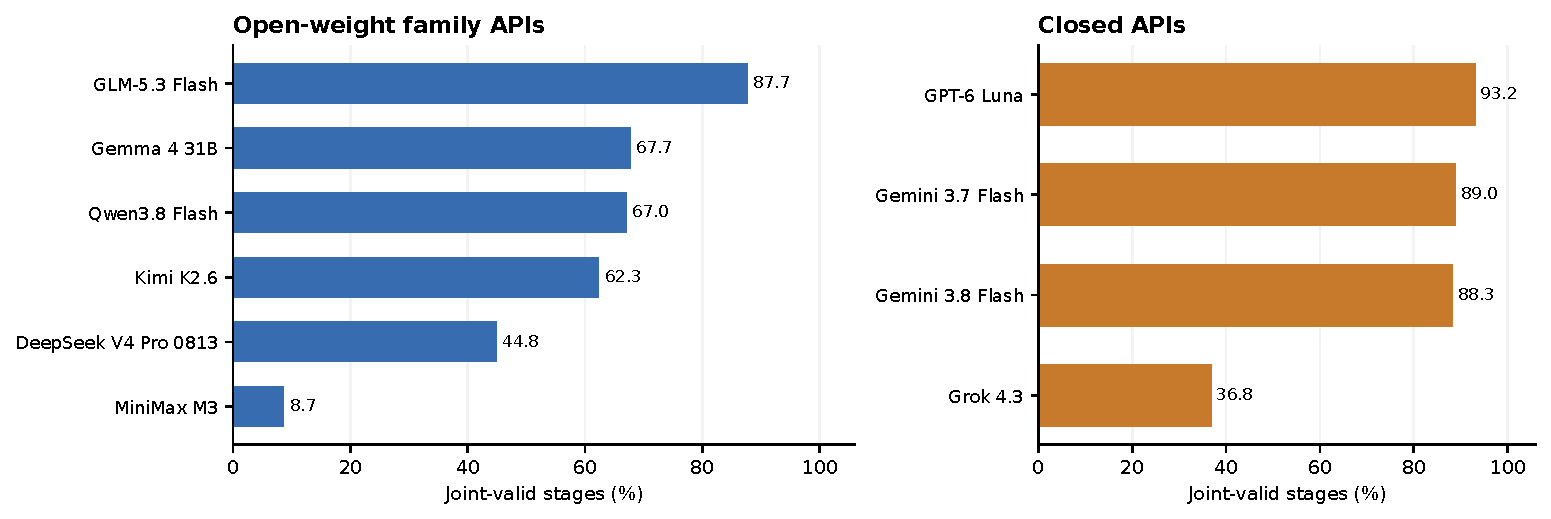
\includegraphics[width=.96\textwidth]{figure_5_validity.pdf}
\caption{Descriptive quality ranking within endpoint-family groups. Scores are valid-stage percentages over 600 stages. Work, time, and adaptation are reported separately and are not included in these bars.}
\end{figure*}

Across the initial, relevant, and irrelevant conditions, unconditional valid counts are 1,479, 862, and 1,532 out of 2,000 each. The conditional related and irrelevant counts are 807 and 1,468 out of 1,479. The difference arises because unconditional update outcomes also include continuations from initially invalid states. Exact per-model counts appear in Table~\ref{tab:counts}.

For one-worker native replay on medium tasks, 121/467 pairs show positive attenuation, 14/467 show nonpositive time savings, and 332/467 show at least proportional savings. The equal-parent mean gap is $-7.9$ points (95\% interval $[-15.6,1.0]$). At four workers the corresponding counts are 108, 27, and 332, with a mean gap of $-6.0$ points. These are different executions of fixed saved decisions. They diagnose timing layers without changing the generated workflow.

The same-pair comparison between four-worker native and online savings gives 41.3 points (24.4--61.1) before removing local admission and 24.2 points (13.9--34.5) afterward. Each statistic averages within a parent before averaging across the 37 eligible parents. Pair counts reflect available matched executions; they are not independent task counts.

Source-aware adaptation estimates average eligible repeats within parents, then use cluster-within-scenario and parent resampling. For Luna, the equal-parent relevant-update estimate is 83.3\% (76.7--89.7); for GLM it is 81.1\% (74.0--87.7). These differ slightly from the pooled conditional rates because a parent with one valid initial repeat receives the same parent weight as a parent with two. The release also provides every pairwise common-support adaptation table. Only eight parent--repeat cells have valid initial outcomes for all ten models, making that common intersection a small descriptive slice.

\section{Related-Work Coverage Evidence}
\label{app:coverage}
\begin{table*}[t]
\centering\small
\setlength{\tabcolsep}{3pt}
\begin{tabular}{lccccc}
\toprule
Evaluation & Executed outcome & Native work vector & Work--time pairing & Relevant updates & Valid-prefix cost\\
\midrule
WorFBench & $\circ$ & -- & -- & -- & --\\
FlowBench / FlowMind & $\checkmark$ & -- & -- & -- & --\\
AgentBoard & $\checkmark$ & -- & -- & -- & --\\
AppWorld & $\checkmark$ & -- & -- & -- & --\\
ClawArena-Team & $\checkmark$ & -- & -- & $\checkmark$ & --\\
OrchBench & $\circ$ & $\circ$ & $\circ$ & -- & --\\
\textbf{WELD} & $\checkmark$ & $\checkmark$ & $\checkmark$ & $\checkmark$ & $\checkmark$\\
\bottomrule
\end{tabular}
\caption{Reported coverage of the operational measurements used here. $\checkmark$: direct coverage; $\circ$: related coverage with a different measurement domain; --: no separately reported protocol of this definition in the inspected version. Native work vector retains heterogeneous execution units. Work--time pairing jointly measures native work and observed time for matched valid workflows. Valid-prefix cost measures new work from a validated completed checkpoint. WorFBench includes downstream execution; OrchBench reports simulated quality, makespan, and tokens. Appendix~\ref{app:coverage} gives the source mapping.}
\label{tab:coverage}
\end{table*}

Table~\ref{tab:coverage} maps reported protocols to the definitions in this paper. WorFBench v3 uses structural matching and includes downstream execution and timing experiments. FlowMind v1 evaluates task execution and reconstructed workflows, with token and tool-use analysis. AgentBoard reports progress and analytical evaluation, while AppWorld verifies application state. ClawArena-Team v2 reports execution-based task scoring, staged updates, permission/modality metrics, and usage analysis. OrchBench v1 evaluates quality, makespan, and token cost with a deterministic simulator. A related result is marked partial when its measurement domain differs from native execution. The table's final column specifically requires incremental cost from a validated completed prefix and a relevant/irrelevant contrast. This mapping concerns the reported measurements, not the theoretical capacity of their environments.

\section{Reproducibility Files}
The companion tables contain all 6,000 stages, all 5,006 initial pairs, component-level work, timing eligibility, prefix audits, adaptation pools, and source-aware sensitivity analyses. Figure scripts use these tables directly. Plans, revisions, observations, physical attempts, and frozen sources are indexed in the research archive. Task cards and evaluator source remain available independently of the run directories. All manuscript counts use the final audit.

\end{document}
